\documentclass{article}
\usepackage{graphicx}
\usepackage{amsmath}
\usepackage{hyperref}
\usepackage[margin=1in]{geometry}
\usepackage{booktabs} 
\usepackage{xcolor}
\usepackage{listings}

\usepackage{float} 

\lstdefinestyle{Python}{
    language=Python,
    basicstyle=\ttfamily\small,
    keywordstyle=\color{blue}\bfseries,
    stringstyle=\color{red},
    commentstyle=\color{gray}\itshape,
    showstringspaces=false,
    numbers=left,
    numberstyle=\tiny,
    stepnumber=1,
    numbersep=5pt,
    frame=single,
    breaklines=true,
    postbreak=\mbox{\textcolor{red}{$\hookrightarrow$}\space}
}

\title{Highly Efficient Geometric Brownian Motion Modeling with QMCPy}
\author{Larysa Matiukha, Aleksei Sorokin, and Sou-Cheng Choi}
\date{\today}
\begin{document}
\maketitle

\section{Introduction}

In this blog post, we demonstrate how to simulate and analyze a Geometric Brownian Motion (GBM) process using QMCPy in Python.
GBM is widely used in finance to model stock prices and other assets. 
We will walk through key code snippets, plots, and insights.

GBM is a continuous stochastic process in which the natural logarithm of its values follows a Brownian motion $[1]$.
Mathematically, it can be defined as follows:
$$\large{S_t = S_0 \, e^{\big(\mu - \frac{\sigma^2}{2}\big)  t + \sigma W_t}}, \label{gbm}$$
where
\begin{itemize}
\item $S_0$ is the initial value, 
\item $\mu$ is a drift coefficient
\item $\sigma$ is a diffusion coefficient  
\item $W_t$ is a (standard) Brownian motion.
\end{itemize}

At any time $t > 0$, $S_t$ follows a log-normal distribution with expected value and variance as follows (see Section 3.2 in $[1]$):
\begin{itemize}
\item
 $E[S_t] = S_0 e^{\mu t}$
\item $\text{Var}[S_t] = S_0^2 e^{2\mu t}(e^{\sigma^2 t} - 1)$
\item   $  
    \text{Cov}(S(t_i), S(t_j)) = S_0^2 e^{\mu(t_i + t_j)} \left(e^{\sigma^2 \min(t_i, t_j)} - 1\right).$
\end{itemize}

GBM is commonly used to model stock prices driving option payoffs. 

\section{GBM object in QMCPy}

GBM in QMCPy inherits from BrownianMotion class $[2, 3]$. 
We can create a simple GBM instance and generate sample paths to see the class in action:

\lstinputlisting[
    style=Python,
    caption={Generating 4 samples from a 2-D GBM using QMCPy},
    label={lst:gbm_qmcpy}
]{code/gbm_qmcpy.py}

The output shows 4-sample paths from a 2-dimensional GBM:
\begin{verbatim}
array([[2.27098076, 1.87407883],
       [0.5370409 , 0.55870756],
       [0.19231031, 0.3744054 ],
       [1.01040524, 0.89379215]])
\end{verbatim}

Let's validate the  theoretical properties by generating a large number of GBM samples and comparing the empirical moments with the theoretical values. Note that the theoretical values match the last values captured in \texttt{qp\_gbm.mean\_gbm} and \texttt{qp\_gbm.covariance\_gbm} for the final time point. The results are reported in Table~\ref{tab1}.

\lstinputlisting[
    style=Python,
    caption={Generating and validating GBM sample moments},
    label={lst:gbm-validation}
]{code/gbm_moments_validation.py}

\begin{table}[t]
\centering
\caption{Theoretical vs Empirical Validation of GBM Properties}
\begin{tabular}{ll}
\hline
\textbf{Statistic} & \textbf{Value} \\
\hline
Sample Mean & 105.134 (Theoretical: 105.127) \\
Sample Variance & 453.062 (Theoretical: 451.029) \\
\hline
Time Vector & [0.2,\; 0.4,\; 0.6,\; 0.8,\; 1.0] \\
Drift ($\mu$) & 0.05 \\
Diffusion ($\sigma$) & 0.20\\
Mean  & [101.005,\; 102.020,\; 103.045,\; 104.081,\; 105.127] \\
Decomposition Type & PCA \\
\hline
\multicolumn{2}{l}{\textbf{Covariance Matrix:}} \\
\multicolumn{2}{l}{
\(
\begin{bmatrix}
81.943 & 82.767 & 83.599 & 84.439 & 85.288 \\
82.767 & 167.869 & 169.556 & 171.260 & 172.981 \\
83.599 & 169.556 & 257.923 & 260.516 & 263.134 \\
84.439 & 171.260 & 260.516 & 352.258 & 355.798 \\
85.288 & 172.981 & 263.134 & 355.798 & 451.029
\end{bmatrix}
\)
} \\
\hline
\end{tabular}
\label{tab1}
\end{table}

\section{GMB vs Brownian Motion}

Below we compare Brownian motion and geometric Brownian motion using the same parameters: $\texttt{drift} = 0$, $\texttt{diffusion} = 1$, $\texttt{initial\_value} = 1$.

First, let's define a utility function that will help us visualize GBM paths with different samplers and parameters:
\lstinputlisting[
    style=Python,
    caption={Function to plot BM and GBM sample paths},
    label={lst:plot-paths}
]{code/plot_paths.py}


Paths of the driftless Brownian motion should fluctuate symmetrically around the initial value (y = 1) and can take negative values, while those of Geometric Brownian Motion remain strictly positive.

\lstinputlisting[
    style=Python,
    caption={Generate 16 BM and 16 GBM sample paths},
    label={lst:gbm_qmcpy}
]{code/bm_gbm_16.py}

\begin{figure}[t!]
\centering
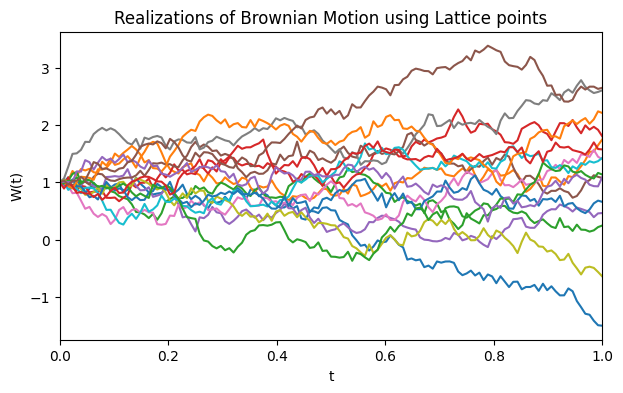
\includegraphics[width=0.49\textwidth]{images/figure_1.png}
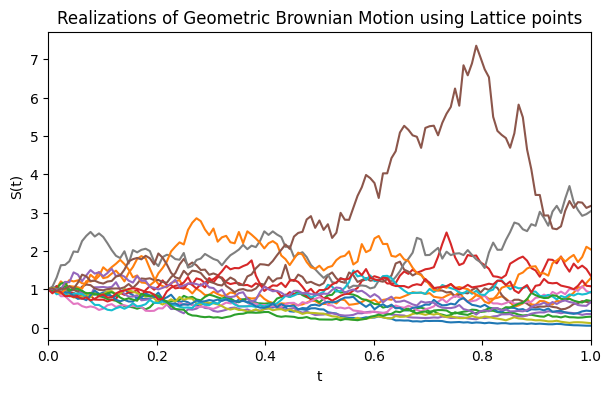
\includegraphics[width=0.49\textwidth]{images/figure_2.png}\\
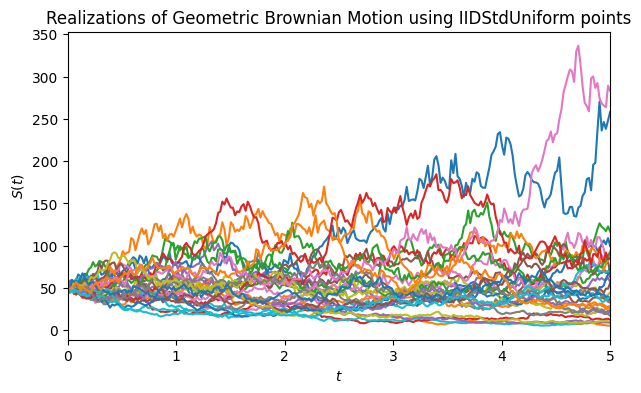
\includegraphics[width=0.49\textwidth]{images/figure_3.png}
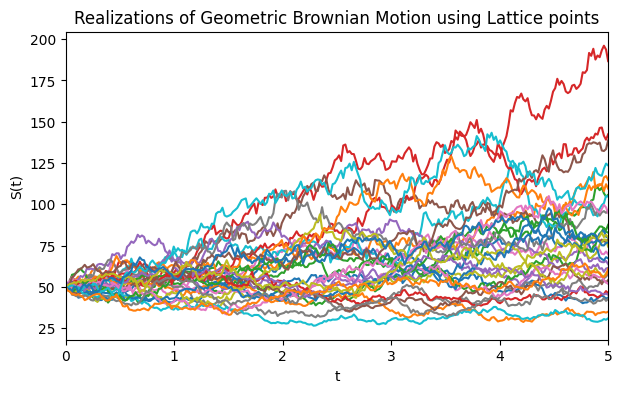
\includegraphics[width=0.49\textwidth]{images/figure_4.png}
\caption{Sample paths of BM and GBM.}
\end{figure}

% \begin{figure}[H]
% \centering
% 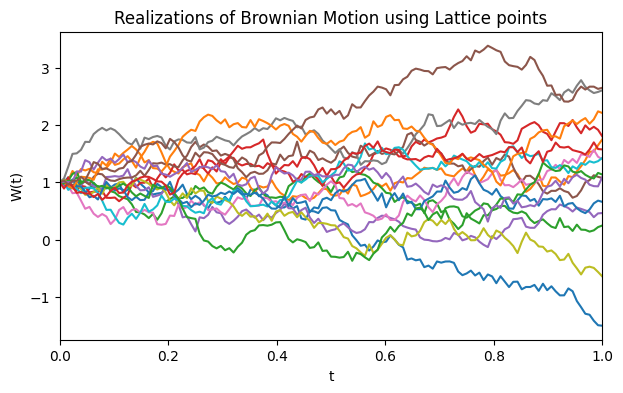
\includegraphics[width=0.49\textwidth]{images/figure_1.png}
% 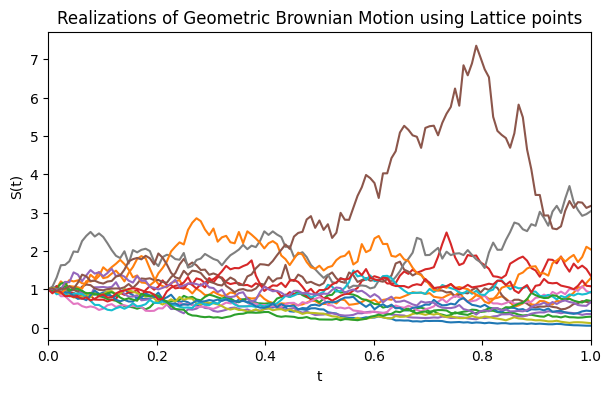
\includegraphics[width=0.49\textwidth]{images/figure_2.png}\\
% 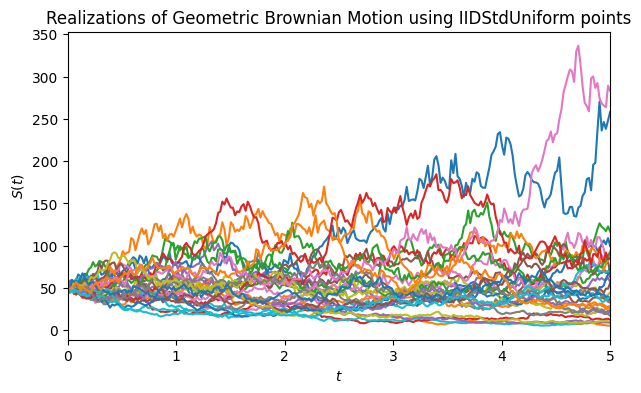
\includegraphics[width=0.49\textwidth]{images/figure_3.png}
% 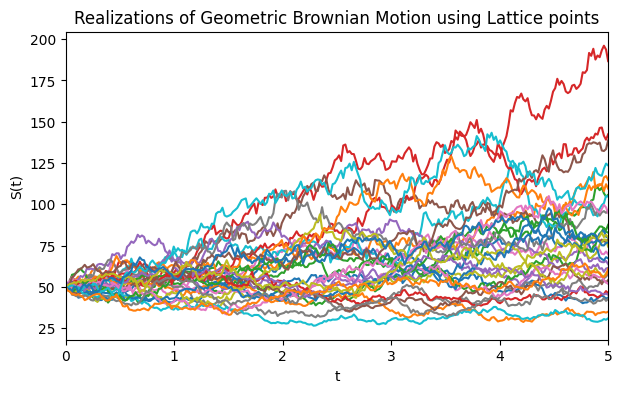
\includegraphics[width=0.49\textwidth]{images/figure_4.png}
% \caption{Sample paths of BM and GBM.}
% \end{figure}

Next, we demonstrate how easily one can swap samplers or change parameters.  For example, to model a stock price
with initial value $S_0=50$, drift $\mu=0.1$, and volatility $\sigma=0.2$ over a 5‐year horizon using IID sampling:
\lstinputlisting[
    style=Python,
    caption={Generate 32 GBM sample paths with IID sampling},
    label={lst:gbm_iid_32}
]{code/gbm_iid_32.py}

Or, to use a low‐discrepancy lattice sampler with the same parameters:
\lstinputlisting[
    style=Python,
    caption={Generate 32 GBM sample paths with lattice sampling},
    label={lst:gbm_lattice_32}
]{code/gbm_lattice_32.py}

% \begin{figure}[H]
% \centering
% 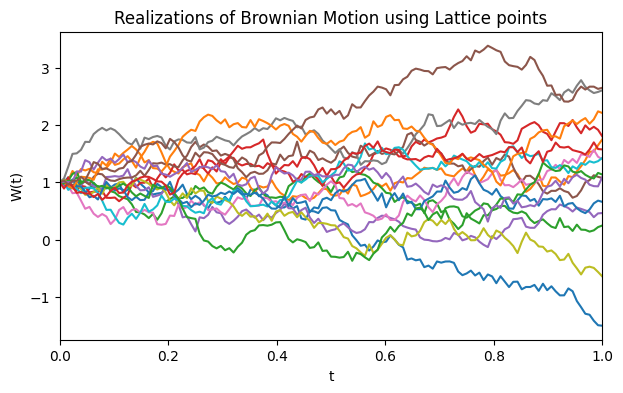
\includegraphics[width=0.49\textwidth]{images/figure_1.png}
% 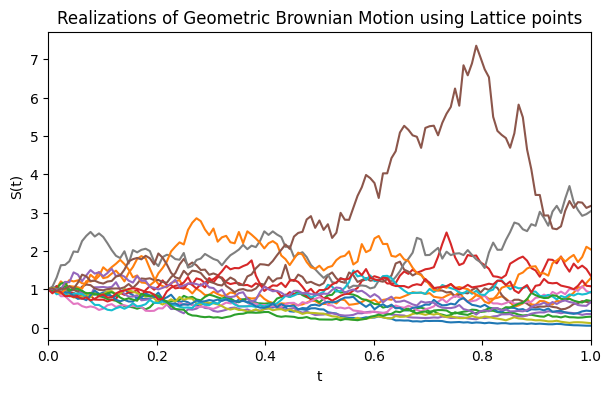
\includegraphics[width=0.49\textwidth]{images/figure_2.png}\\
% 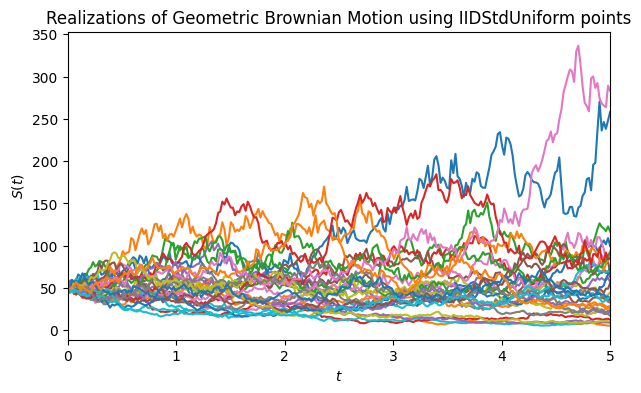
\includegraphics[width=0.49\textwidth]{images/figure_3.png}
% 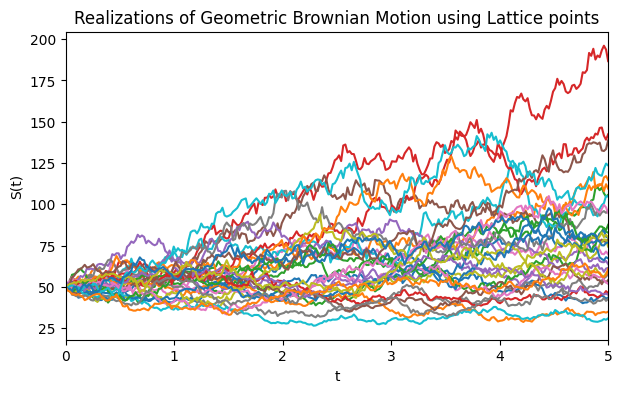
\includegraphics[width=0.49\textwidth]{images/figure_4.png}
% \caption{Sample paths of BM and GBM.}
% \end{figure}


\section{QuantLib vs QMCPy Comparison}

In this section, we compare QMCPy's GeometricBrownianMotion implementation with the industry-standard QuantLib library [6] to validate its accuracy and performance. The numerical results are summarized in Table~\ref{tab2}.
\lstinputlisting[
    style=Python,
    caption={Function to generate GBM paths with QuantLib},
    label={lst:quantlib}
]{code/quantlib.py}


\begin{figure}[t!]
\centering
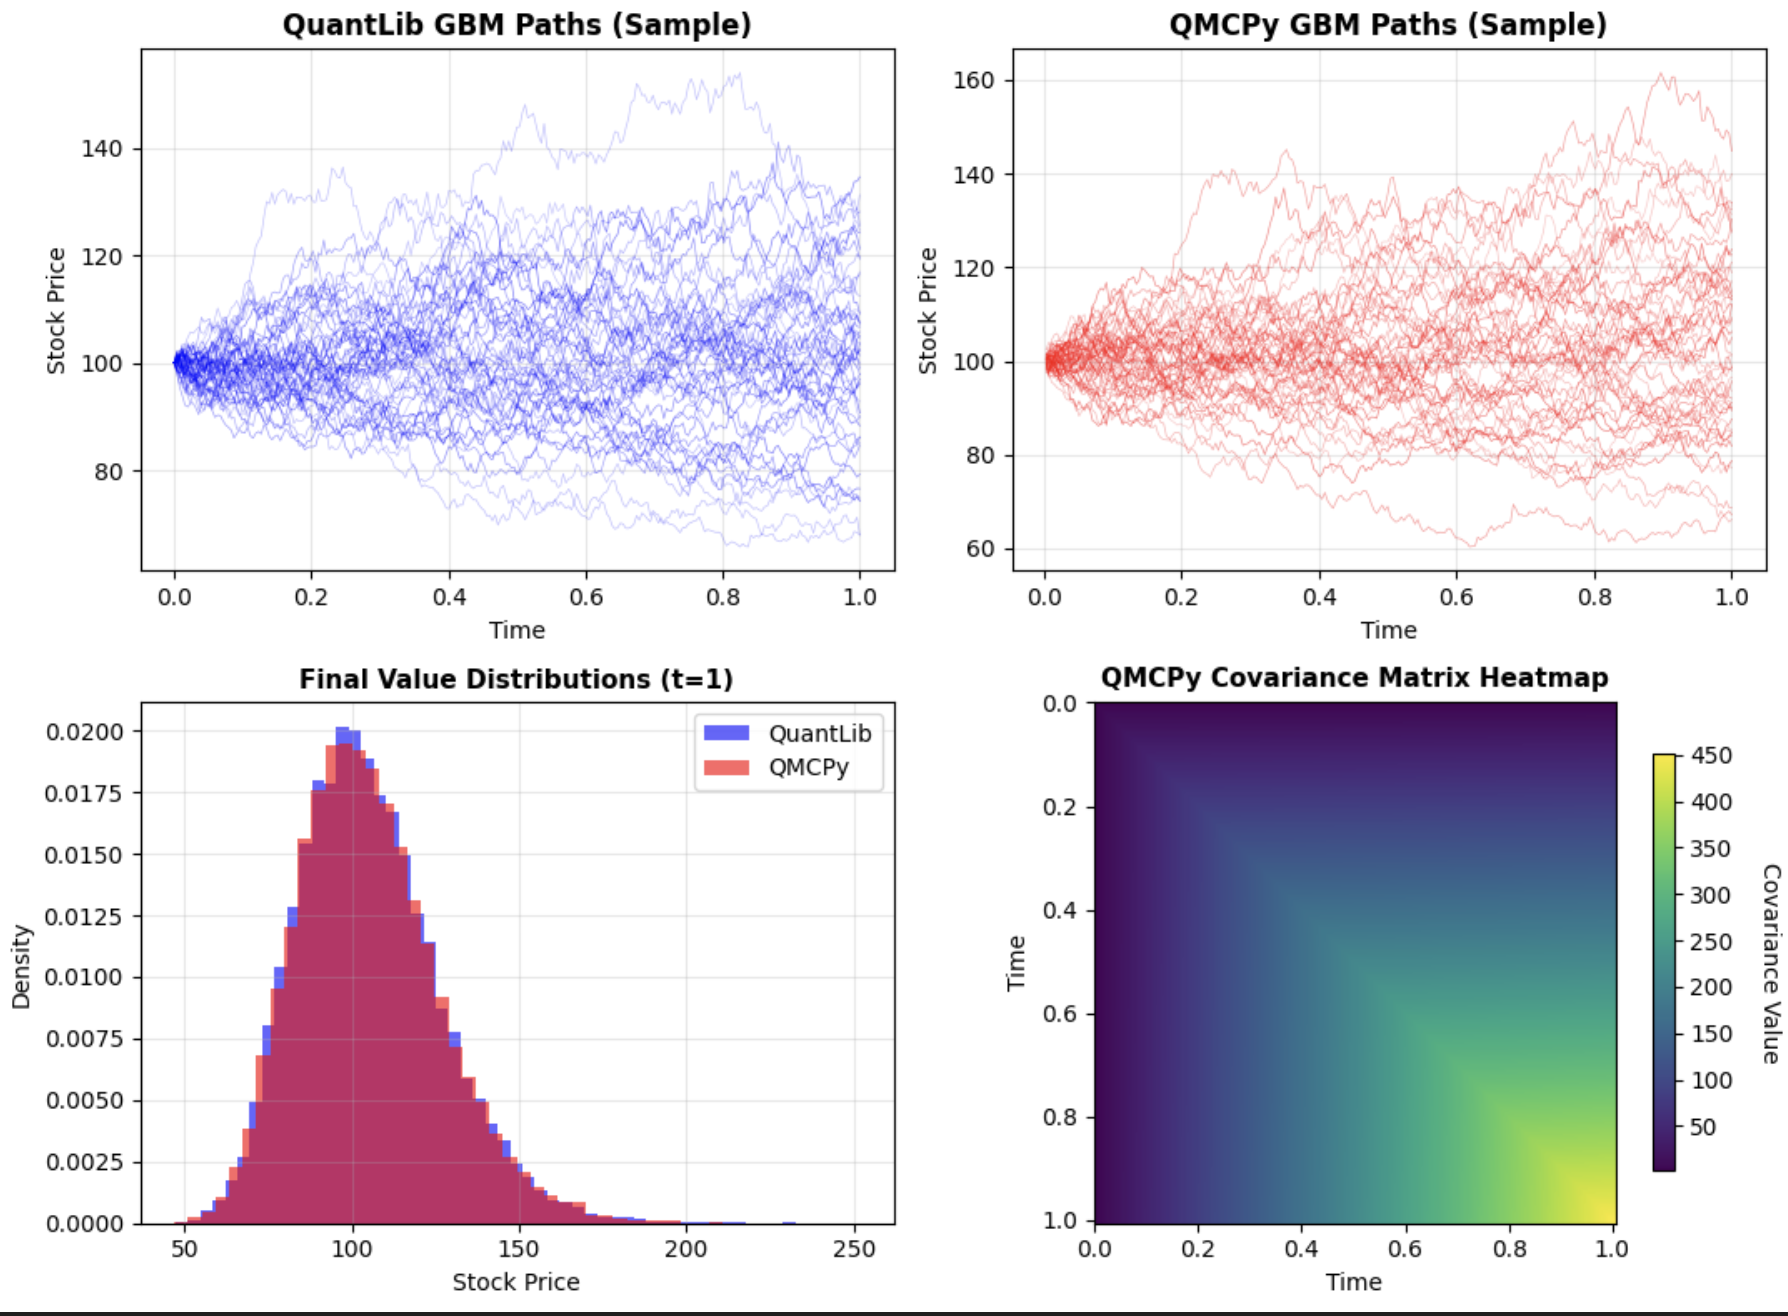
\includegraphics[width=1\textwidth]{images/figure_5.png}
\caption{QMCPy vs QuantLib comparison. The heatmap displays the covariance matrix with time 0 at the top of the y-axis, allowing direct visual comparison with the numerical values in the  matrix such as the one shown in Table~\ref{tab1}.}
\end{figure}

\begin{table}[t]
\centering
\caption{QuantLib vs QMCPy: QMCPy is 3.4 times faster than QuantLib in generating thousands of paths.}
\begin{tabular}{lccc}
\toprule
\textbf{Method} & \textbf{Mean} & \textbf{Std. Dev.} & \textbf{Time (s)}   \\
\midrule
QuantLib & 105.10 & 21.11 & 0.819  \\
QMCPy & 105.13 & 21.25 & 0.239  \\
Theoretical & 105.13 & 21.24 & ---  \\
\bottomrule
\end{tabular}
\label{tab2}
\end{table}

Both libraries produce statistically equivalent GBM simulations that match theoretical values. QMCPy typically runs 2-4 times faster due to vectorized operations, making it excellent for research and high-performance applications. QuantLib remains the industry standard for production systems requiring comprehensive  support for financial modeling and risk management.


\section{Internals}

The \texttt{GeometricBrownianMotion} class in QMCPy is engineered for speed, robustness, and mathematical correctness. Its design leverages object-oriented inheritance and vectorized operations, resulting in both flexibility and high performance.
\texttt{GeometricBrownianMotion} inherits from \texttt{BrownianMotion} which itself inherits from \texttt{Gaussian}. This layered design allows the GBM class to reuse and extend efficient implementations for Gaussian random vectors and Brownian motion increments.
The constructor rigorously checks input parameters (e.g., positivity of initial value and diffusion, valid decomposition type), ensuring mathematical integrity and preventing runtime errors.

The class uses vectorized NumPy operations to generate entire arrays of GBM paths in a single call, minimizing Python loops and maximizing computational throughput. Sample generation proceeds in two stages:
\begin{enumerate}
\item 
The parent class \texttt{BrownianMotion} generates standard Brownian motion sample paths using the specified sampler (e.g., low-discrepancy lattice, IID uniform), with drift and diffusion handled in the mean and covariance structure.
\item  The GBM class transforms the BM samples via the exponential mapping    \eqref{gbm}, performed in a fully vectorized fashion, ensuring that thousands of paths can be efficiently simulated.
\end{enumerate}
The class computes and stores the theoretical mean and covariance matrices for GBM at initialization, which can be used for validation and theoretical comparisons. Both mean and covariance are calculated using analytical formulas, leveraging \href{https://numpy.org/devdocs/user/basics.broadcasting.html}{NumPy’s broadcasting} for efficient computations. (Briefly, broadcasting in NumPy allows arithmetic operations between arrays of different shapes by automatically expanding the smaller array to match the shape of the larger array.)

 The Gaussian and Brownian‐motion classes both implement both Cholesky and PCA factorization of the covariance matrix
\[
\Sigma \;=\; L\,L^{\!\top}
\quad\text{and}\quad
\Sigma \;=\; P\,D\,P^{\!\top},
\]
respectively.  In the Cholesky method, one computes the lower‐triangular $L=\operatorname{chol}(\Sigma)$ and obtains correlated increments via $X=L\,Z$, where $Z\sim\mathcal{N}(0,I)$.  In the PCA approach, one first diagonalizes $\Sigma=PDP^{\!\top}$, then forms $X = P\,D^{1/2}\,Z$.  By default PCA is used for its superior numerical stability in high dimensions and slightly lower cost when many eigenvalues are near zero.  These correlated normals feed directly into the GBM update
\[
S(t+\Delta t) \;=\; S(t)\,\exp\!\Bigl((\mu - \tfrac12\sigma^2)\Delta t \;+\;\sigma\sqrt{\Delta t}\,X\Bigr),
\]
ensuring that the simulated paths respect the intended covariance structure and remain strictly positive (with strict‐positivity checks raising warnings or errors if violated).



\begin{thebibliography}{6}

\bibitem[1]{glasserman2003}
Glasserman, P. (2003). \textit{Monte Carlo Methods in Financial Engineering} (2nd ed.). Springer.

\bibitem[2]{choi2022}
Choi, S.-C. T., Hickernell, F. J., Jagadeeswaran, R., McCourt, M. J., \& Sorokin, A. G. (2022).
Quasi-Monte Carlo Software. In A. Keller (Ed.), \textit{Monte Carlo and Quasi-Monte Carlo Methods}.
Springer International Publishing.

\bibitem[3]{qmcpy2023}
Choi, S.-C. T., Hickernell, F. J., Jagadeeswaran, R., McCourt, M. J., \& Sorokin, A. G. (2025).
QMCPy: A quasi-Monte Carlo Python Library (Versions 1–1.6.2.1).

\bibitem[4]{hull2017}
Hull, J. C. (2017). \textit{Options, Futures, and Other Derivatives} (10th ed.). Pearson.

\bibitem[5]{ross2014}
Ross, S. M. (2014). \textit{Introduction to Probability Models} (11th ed.). Academic Press.

\bibitem[6]{quantlib}
QuantLib Development Team. (n.d.). \textit{QuantLib: A free/open-source library for quantitative finance} (Version 1.38).
Retrieved from \url{https://www.quantlib.org}.

\end{thebibliography}


 

\end{document}